\section{Architektur}

Munin verwendet eine sogenannte Master-Node-Architektur, siehe Abbildung \ref{master-munin}.
Hierbei emittelt jeder Rechner seine Messwerte selbst und der Master holt sich diese Daten mittels diverser Agenten, den sogenannten Munin-Nodes, ab.
Deshalb wird der Master lediglich zur Verarbeitung der Überwachungsdaten genutzt.

\begin{figure}[ht]
	\centering
	   \fbox{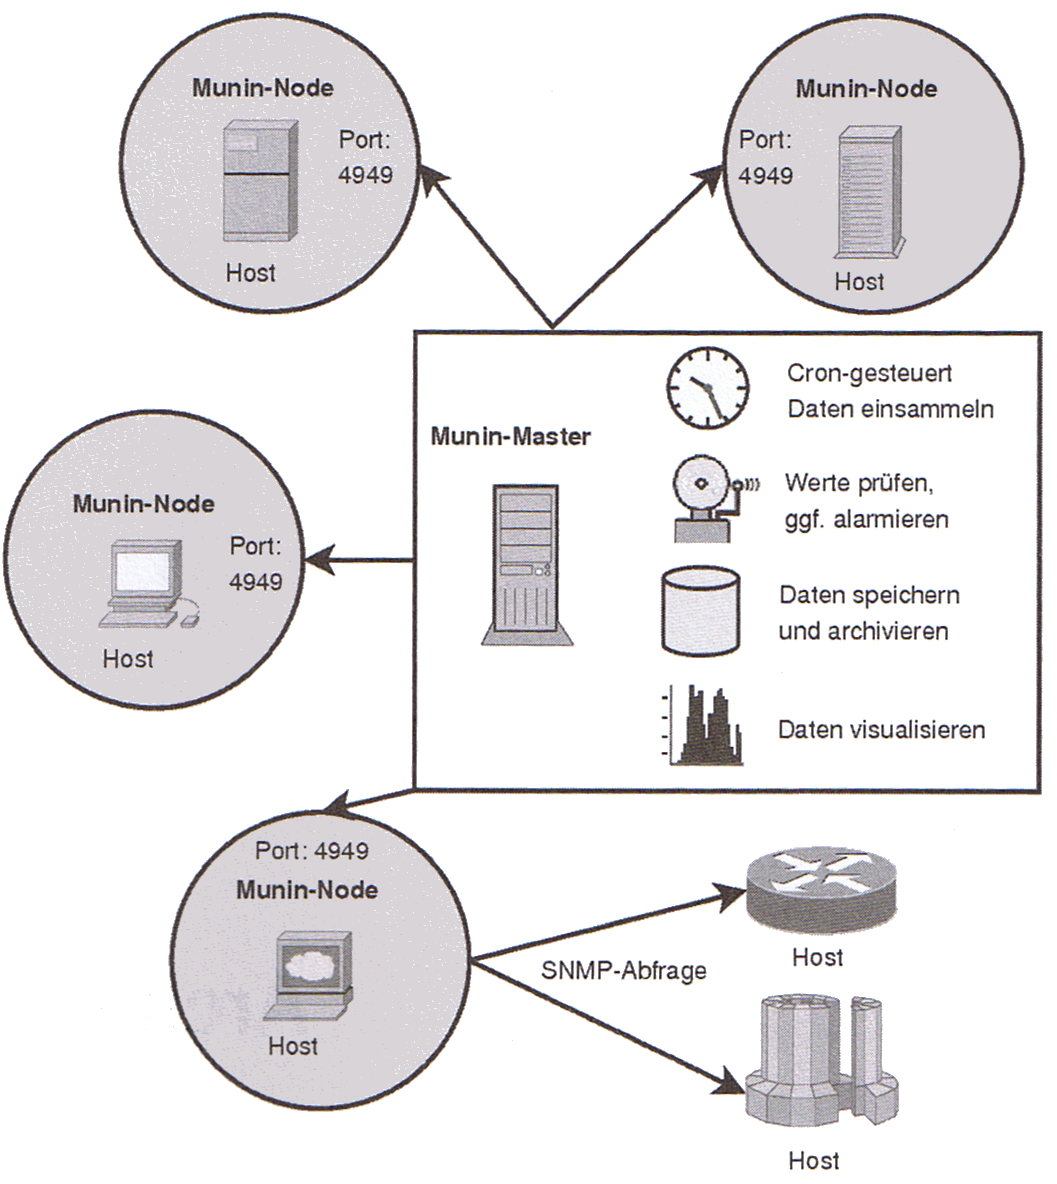
\includegraphics[width=0.85\textwidth]{bilder/master.png}}
		\caption[Munin Master-Node-Konzept]{Munin Master-Node-Konzept\protect\footnotemark}
		\label{master-munin}
\end{figure}
\footnotetext{Quelle: \cite{Mu08} S. 20}

Der Munin-Master ist kein Daemon, sondern besteht aus Skripten, die in regelmäßigen Zeitabstanden als Cron-Job ablaufen:
\begin{itemize}
\item \pictext{munin-update} dient zum Abrufen der Messwerte bei den zu überwachenden Munin-Nodes. Hierbei wird auch die Datenbank aktualisiert oder ggf. erzeugt.
\item \pictext{munin-limits} vergleicht die Messwerte mit ggf. vorgegebenen Schwellwerten und versendet bei Bedarf Benachrichtigungen, wenn Werte das Warnlevel überschreiten, in kritische Bereich gelangen oder wenn Entwarnung gegeben werden kann.
\item \pictext{munin-graph} erzeugt die Munin-Graphen.
\item \pictext{munin-html} dient zum Erstellen der HTML-Seiten der Munin-Übersicht.
\end{itemize}

Standardmäßig werden diese Skripte im fünf Minuten Rythmus aufgerufen.
Dabei baut der Munin-Master viele parallele - im Ausgangszustand unverschlüsselte - TCP-Verbindungen zu den diversen Node-Hosts auf.

Zusätzlich wird für den Betrieb des Munin-Masters auf einem Rechner folgende vorab konfigurierte Software vorausgesetzt:

\begin{itemize}
\item einen Webserver, der Zugang zu den Graphen verschafft.
\item ein Programm mit dem sich die Warnmeldungen versenden lassen. Beispielsweise einen SMTP-Server oder einen Nagios Service Check Acceptor (NSCA), der dafür sorgt, dass der Nagios-Server Alarm schlägt.
\item Werkzeuge und Bibliotheken des \textit{RRDtool}-Projekts\footnote{http://oss.oetiker.ch/rrdtool/} zur Speicherung der Daten und zum Zeichnen der Munin-Graphen.
\end{itemize}


\subsection{Einsammeln der Daten}
Das periodisch ausgeführte Perlskript \pictext{munin-update} kümmert sich um das Abholen neuer Messwerte von den Nodes.
Dazu wird als Erstes die Datei \pictext{munin.conf} geparst, um die zu überwachenden Nodes zu ermitteln.

Ein Eintrag für einen Node-Host in dieser Datei sieht folgendermaßen aus:


\begin{lstlisting}[captionpos=b, caption=Beispielhafte Definition eines Munin-Nodes, label=nodedef, breaklines = true, language=bash]
[munin.example.net]
	address 			localhost
	port				6088
	df.warning			20
	df.critical			10
	contacts			paul
	ping_unilabad.contacts		lang
\end{lstlisting}

Der String in den eckigen Klammern wird als Identifikationsnamen für den Host verwendet und dieser Node wird auch im Webinterface unter diesem Namen aufgelistet.

Das Attribut \textit{address} gibt die IP-Adresse des zu überwachenden Hosts an und mit \textit{port} kann ein vom Standardport (4949) abweichender Port angegeben werden.

Die einzelnen Schwellwerte der verschiedenen Plugins werden auch in diesem Eintrag angegeben, wenn sie von den vorkonfigurierten Werten abweichen sollen.
Dafür wird der Name des Plugins mit den Suffixen \textit{.warning} und \textit{.critical} für die jeweiligen Schwellwerte gesetzt.
Im obigen Beispiel wird \pictext{df} für den freien Festplattenspeicherplatz mit dem Schwellwert von 20\% für Warnungen und 10\% als kritischen Wert für den Host definiert.

Unter dem Attribut \textit{contacts} werden die Kontaktnamen angegeben, die bei einer Überschreitung eines Schwellwerteres kontaktiert werden sollen.
Hierbei gibt es zu sagen, dass diese Überschreitung bei egal welchem Plugin für die Benachrichtigung dieser Kontakte führt.

Soll ein Kontakt nur bei einem bestimmten Plugin benachrichtigt werden, muss es analog zu der Schwellwertdefinition mit dem Pluginnamen und dem Suffix \textit{.contacts} explizit angegeben werden. Hier wird der Kontakt \textit{lang} nur bei einer Überschreitung des Plugins \textit{ping\_unilabad} benachrichtigt.
Bei diesem Plugin wird der Host \textit{unilabad} mit einem Ping überwacht.
Für weitere Details zu dieser Art von Plugin siehe Kapitel \ref{wildcard}.

Weiterhin lässt sich einstellen, dass ein Kontakt generell nur bei kritischen Werten benachrichtigt werden soll.
Die Kontakte müssen zuvor in der \\ \pictext{munin.conf} definiert werden.

Nach der Ermittlung der Nodes werden die Hosts in der Regel parallel nach den neuen Messwerten abgefragt.
Hierfür erzeugt Munin  für jeden in der Konfigurationsdatei angegebenen Rechnern einen eigenen Prozess.
Das parallele Abarbeiten hat den Vorteil, dass die Abfrage nicht bis zum Timeout hängen bleibt, wenn ein einzelner Munin-Node nicht erreichbar ist.
Jedoch verschlingt das Erzeugen eines eigenen Prozesses für jeden Node bei vielen zu überwachenden Rechnern viele Ressourcen, so dass bei größeren Umgebungen viel Arbeitsspeicher und schnelle Multicoreprozessoren unabdingbar sind.

Ein beispielhafte Ausführung eines Munin-Plugins für die Plattenbelegung gibt folgende Werte zurück:

\begin{figure}[ht]
	\centering
	   \fbox{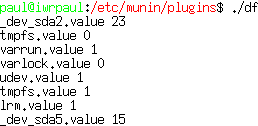
\includegraphics[width=0.6\textwidth]{bilder/df-munin.png}}
		\caption{Beispielhafte Ausführung eines Munin-Plugins}
		\label{df-munin}
\end{figure}
\newpage
Wenn man diese Werte mit den realen Werten vergleicht, erkennt man, dass das Munin-Plugin einfach die Prozentwerte des verbrauchten Speicherplatzes als Wert verwendet.

\begin{figure}[ht]
	\centering
	   \fbox{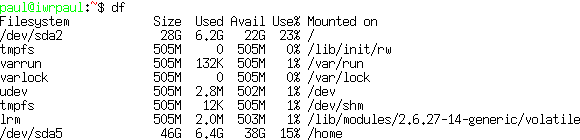
\includegraphics[width=0.85\textwidth]{bilder/df.png}}
		\caption{Reale Werte des Systemtools \textit{df}}
		\label{df}
\end{figure}

Aus diesen Werten erstellt \pictext{munin-graph} automatisch folgenden Graphen:

\begin{figure}[ht]
	\centering
	   \fbox{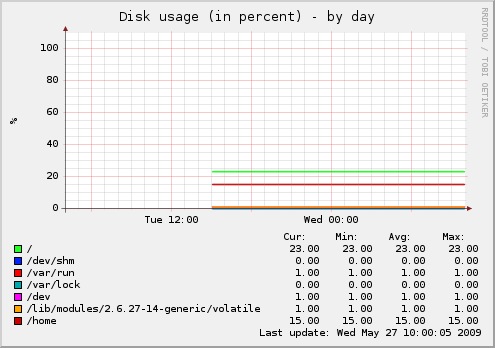
\includegraphics[width=0.85\textwidth]{bilder/df-graph.png}}
		\caption{Visualisierung der Werte des Munin-Plugins \textit{df}}
		\label{df-graph}
\end{figure}

Die über das Netzwerk ermittelten Werte landen nach entsprechender Bearbeitung in RRD-Dateien. 
Im Skript \pictext{munin-update} ist fest eingetragen, welche zeitliche Auflösung die Datenbasis und dadurch auch die Munin-Graphen aufweisen.

Das bedeutet, dass für einen Messpunkt in der Wochenübersicht 30 Minuten - also sechs Messwerte - benötigt werden und für die Monatübersicht werden bereits 48 Messpunkte bzw. zwei Stunden benötigt. Siehe hierfür Tabelle \ref{timeres-tab}.

\begin{table}[!htbp]
\centering
%\begin{twoparttable}
\begin{tabular}{l l}
%\hline
\textbf{Alter der Daten } \hspace{10 mm} & \textbf{Auflösung} \hspace{10 mm} \\
\hline
%\textit{features} & complete\tnote{1} & complete\tnote{1} \\
%\hline
bis zu 30 Stunden & 5 Minuten  \\
\hline
bis zu 9 Tagen & 30 Minuten \\
\hline
bis zu 45 Tagen & 2 Stunden \\
\hline
bis zu 450 Tagen & 1 Tag \\
%\hline
\bottomrule
\end{tabular}
\caption[Zeitliche Auflösung der Datenbasis]{Zeitliche Auflösung der Datenbasis\protect\footnotemark}
\label{timeres-tab}
%\end{twoparttable}
\end{table}
\footnotetext{Quelle: \cite{Mu08} S. 24}


In der Abbildung \ref{4times} konnte der \pictext{munin-node} noch keinen kompletten Tag Messwerte sammeln, weshalb die Jahresübersicht noch keine Messwerte liefern kann und nur mit dem Platzhalterwert \textit{nan} (für nicht defniert) aufgefüllt ist.

\begin{figure}[ht]
	\centering
	   \fbox{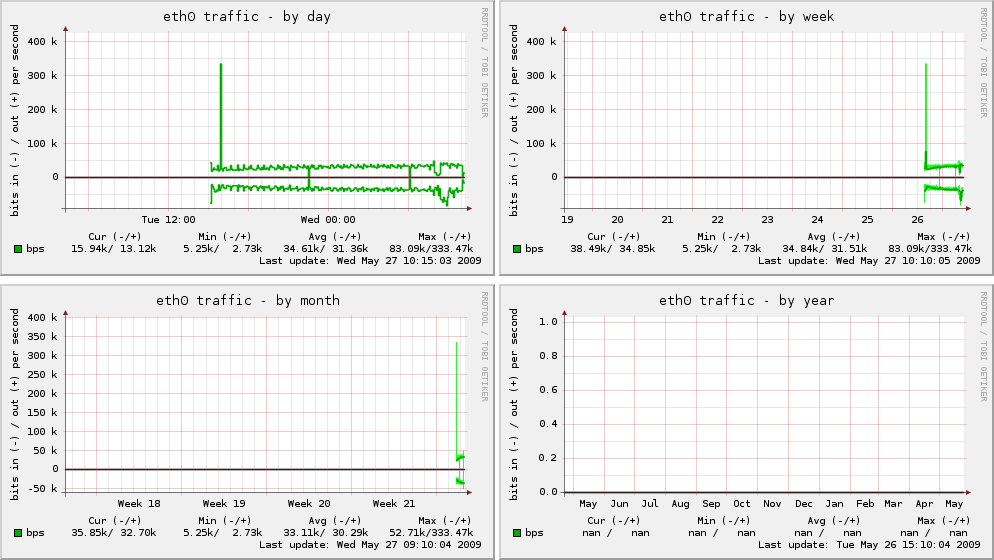
\includegraphics[width=0.9\textwidth]{bilder/4times.png}}
		\caption{Visualisierung der Messwerte in verschiedenen Zeitauflösungen}
		\label{4times}
\end{figure}



\subsection{Round-Robin-Datenbanken}
Round-Robin-Datenbanken sind nicht mit bekannten Datenbanksystemen vergleichbar, da sie in einem proprietären, binären Dateiformat vorliegen.
Daher scheidet der Zugriff per SQL, Texteditor oder über einen Netzwerkport aus.
Um auf Round-Robin-Datenbanken zuzugreifen müssen die dafür entwickelten RRD-Tools verwendet werden.
Diese nehmen die aktuellen Messwerte entgegen und schreiben für jeden Messinterval einen Wert in eine Binärdatei.
Aus dem gesammeltem Datenbestand können dann die Werte visualisiert oder Statistiken erzeugt werden.
Dieser Datenbestand besteht aus sogenannten Round-Robin-Archives.
Dabei handelt es sich um Ableitungen aus den Primärdateien, die mit Hilfe statistischer Auswertungen ermittelt und für die festgelegten Zeitintervalle komprimiert werden.
Die gesamte Anzahl der gespeicherten Datenwerte steht bereits bei der Erzeugung der RRD fest.
Da auch zu Beginn alle Werte mit Platzhaltern aufgefüllt werden, bleibt die Größe einer RRD über die Zeit gleich, siehe Abbildung \ref{rrd-munin}.

\begin{figure}[ht]
	\centering
	   \fbox{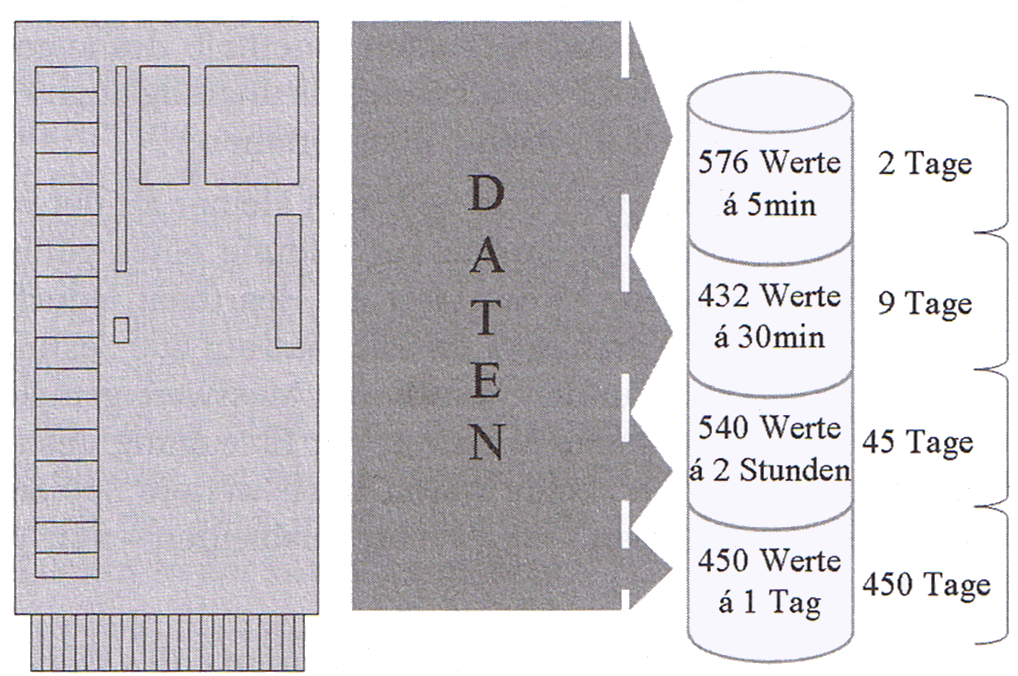
\includegraphics[width=0.76\textwidth]{bilder/rrd.png}}
		\caption[Modell der Round-Robin-Datenbanken]{Modell der Round-Robin-Datenbanken\protect\footnotemark}
		\label{rrd-munin}
\end{figure}
\footnotetext{Quelle: \cite{Mu08} S. 38}

Munin verwendet dieses RRAs als hochauflösende Archive, die die Messwerte des aktuellen Tages, eine etwas komprimierte Fassung zur Darstellung der Daten der laufenden Woche sowie - noch stärker komprimiert - die Daten für den aktuellen Monat und das Jahr enthalten.
%Siehe hierfür Abbildung [?].
Die Komprimierung wird so realisiert, dass Mittelwerte aus der feineren Zeitauflösung errechnet werden und zusätzlich noch spezielle Archivierungsregeln beim Erstellen der RRD-Datei berücksichtigt werden.

Aus diesen Datensätzen mit unterschiedlichen Zeitauflösungen erstellt Munin automatisch Graphen über die entsprechenden Zeiträume, siehe Abbildung \ref{all4}.

\begin{figure}[ht]
	\centering
	   \fbox{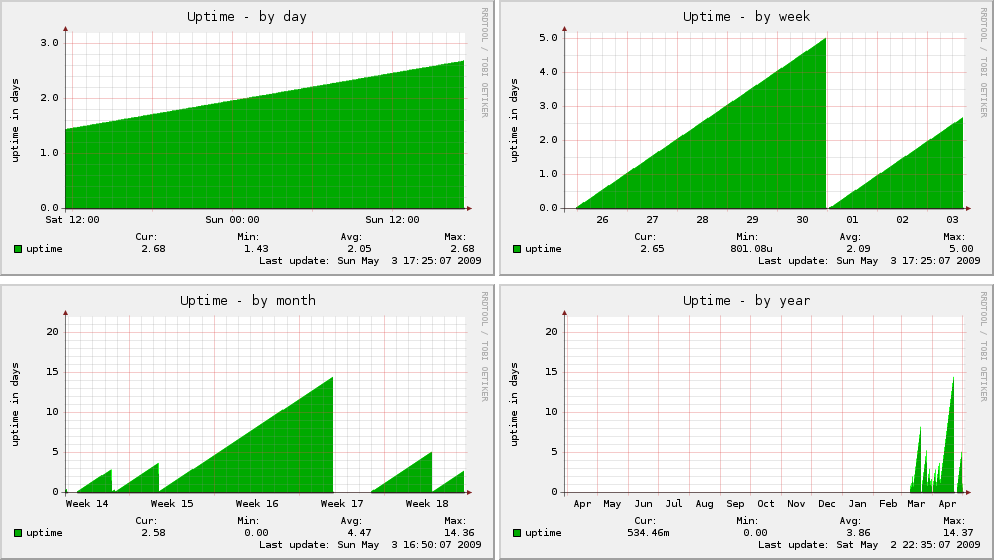
\includegraphics[width=0.95\textwidth]{bilder/all4.png}}
		\caption{Übersicht der \textit{Uptime}}
		\label{all4}
\end{figure}

\newpage

\subsection{Einbindung und Konfiguration der Plugins}
\label{plugins}
Munin bringt bereits eine Sammlung von Plugins bei der Installation mit.
Diese befinden sich in einem Bibliotheksverzeichnis.
Wenn diese Plugins verwendet werden sollen um einen Node zu überwachen, müssen sie in einem Service-Verzeichnis verlinkt sein, damit der Daemon \pictext{munin-node} darauf zugreifen kann.
Dieser Daemon muss sich auf dem zu überwachenden Host befinden und dient als "`Agent"' für den Munin-Master, da der Daemon auf seinem Port nach Aufforderungen durch den Master horcht.
Ein solcher Daemon ist für Linux und für Windows verfügbar, wobei der für Windows weniger Funktionen bietet.
Die einzelnen Tests laufen auf den Nodes unabhängig von der Abfrage des Masters.
Wenn der Master die aktuellen Daten nicht abholt, wird dieser Datenbestand durch die neuen Informationen ausgetauscht und werden bei der nächsten Anfrage an den Master gesendet.

Auf den Graphen im Webinterface wird dieser Zeitraum als Lücke dargestellt, siehe Abbildung \ref{gap}.

\begin{figure}[ht]
	\centering
	   \fbox{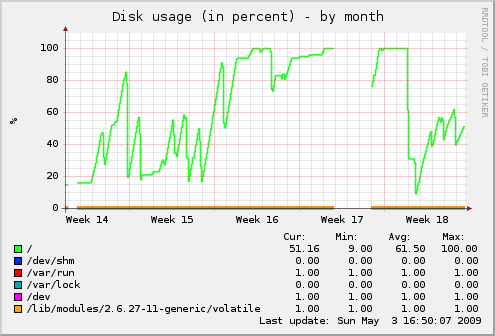
\includegraphics[width=0.852\textwidth]{bilder/gap.png}}
		\caption{Fehlende Messwerte werden als Lücke dargestellt}
		\label{gap}
\end{figure}

Der \pictext{munin-node}-Daemon kannn so konfiguriert werden, dass er nur auf Anfragen von einer bestimmten IP reagiert, einen anderen Port verwendet oder nur auf einer bestimmten IP lauscht.

Damit der Daemon weiss, welche Daten er liefern muss, wird das zuvor erwähnte Service-Verzeichnis verwendet.
Hier werden Verlinkungen zu den eigentlichen Plugins gespeichert.
Eine beispielhafte Verlinkung wird in Abbildung \ref{lns} gezeigt.

\begin{figure}[ht]
	\centering
	   \fbox{
\includegraphics[width=0.85\textwidth]{bilder/lns.png}}
		\caption{Beispielhafte Verlinkung eines Munin-Plugins}
		\label{lns}
\end{figure}

\subsubsection{Wildcard-Plugins}
\label{wildcard}
Falls der Name des Plugins mit einem Unterstrich endet, handelt es sich um ein sogenanntes \textit{Wildcard}-Plugin.
Solche Plugins erwarten in der Bezeichnung des Links spezifische Parameter für die Ausführung der Tests.

Beispielsweise verwendet das zuvor verwendete Plugin \textit{ping\_} als Parameter den Namen oder die IP-Adresse des anzupingenden Hosts.
Die Verlinkung aus dem Bibliotheksverzeichnis in das Service-Verzeichnis würde dann folgendermaßen ausschauen:
\begin{figure}[ht]
	\centering
	   \fbox{
\includegraphics[width=0.85\textwidth]{bilder/lnw.png}}
		\caption{Beispielhafte Verlinkung eines Wildcard-Plugins}
		\label{lnw}
\end{figure}

Hier wird der Host \textit{localhost} angepingt und diese Daten auf dem Master gespeichert und später in einem Graphen visualisiert.

\newpage

\subsubsection{SNMP-Plugins}
Es ist auch möglich Informationen über den zu überwachenden Host in Erfahrung zu bringen, ohne, dass ein \pictext{munin-node}-Daemon auf dem Host installiert ist.
Dies wird durch das Simple Network Management Protocol (SNMP) realisiert.
Durch SNMP kann auf die strukturierte Datenhaltung der MIB in den entfernten Netzwerkknoten zugegriffen werden.
\begin{quote}"`Die Management Information Base (MIB) dient als SNMP-Informations-struktur und besteht aus einem hierarchischen, aus Zahlen aufgebauten Namensraum. Ähnliche Struktur wie andere hierarchische Verzeichnisdiensten wie DNS oder LDAP."'\end{quote}
\begin{flushright}
Quelle: \cite{Barth08} S.233
\end{flushright}

Die MIB-Struktur ist folgendermaßen aufgebaut:

\begin{figure}[ht]
	\centering
	   \fbox{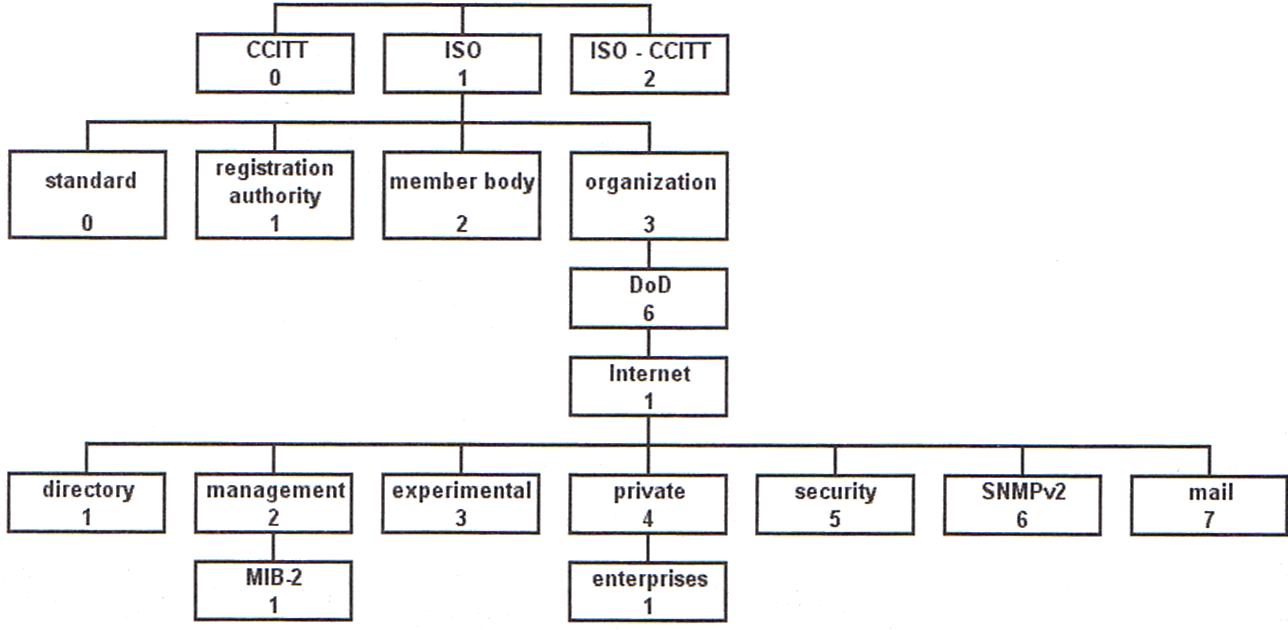
\includegraphics[width=0.95\textwidth]{bilder/mib.png}}
		\caption[Struktur der Management Information Base (MIB)]{Struktur der Management Information Base (MIB)\protect\footnotemark}
		\label{munin-mib}
\end{figure}
\footnotetext{Quelle: \cite{Mu08} S. 156}
Dadurch können die SNMP-Plugins den gewünschten Wert über das Netzwerk abfragen, ohne, dass ein lokal auf dem Munin-Node installiertes Programm notwendig ist.

\newpage

Einen beispielhaften Zugriff auf SNMP-fähige Geräte wird in Abbildung \ref{munin-snmp} gezeigt.

\begin{figure}[ht]
	\centering
	   \fbox{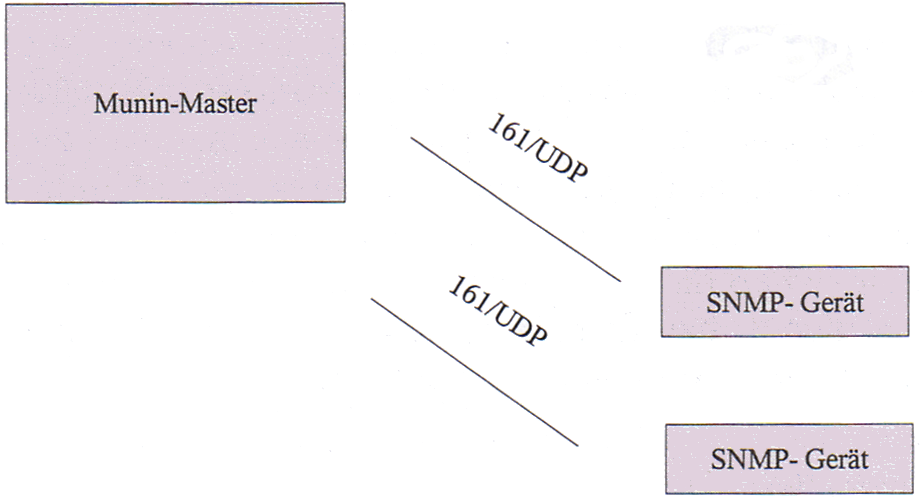
\includegraphics[width=0.85\textwidth]{bilder/snmp.png}}
		\caption[Beispielhafter Zugriff auf SNMP-fähige Geräte]{Beispielhafter Zugriff auf SNMP-fähige Geräte\protect\footnotemark}
		\label{munin-snmp}
\end{figure}
\footnotetext{Quelle: \cite{Mu08} S. 156}

Munin verwendet für SNMP-Plugins eine besondere Namenskonvention.
Alle Plugins dieser Art besitzen den Präfix \textit{snmp\_} auf den die IP-Adresse des SNMP-fähigen Gerätes folgt.
Im folgenden Beispiel wird die Plattenbelegung eines entfernten Knotens überwacht.

\begin{figure}[ht]
	\centering
	   \fbox{
\includegraphics[width=0.85\textwidth]{bilder/snmp-simple.png}}
		\caption{Beispielhafte Verlinkung eines SNMP-Plugins}
		\label{snmp-simple}
\end{figure}

Auch bei diesen SNMP-Plugins gibt es Wildcard-Plugins.
Dabei wird als Suffix im unteren Beispiel der zweite Netzwerkport eines SNMP-fähigen Switches nach Paketfehler abgefragt.

\begin{figure}[ht]
	\centering
	   \fbox{
\includegraphics[width=0.85\textwidth]{bilder/snmp-complex.png}}
		\caption{Beispielhafte Verlinkung eines Wildcard-SNMP-Plugins}
		\label{snmp-complex}
\end{figure}

\newpage

Munin liefert unter anderem folgende SNMP-Plugins mit:

\begin{itemize}
\item \textit{snmp\_\_df} überwacht die Plattenbelegung.
\item \textit{snmp\_\_if\_} ermittelt den Netzwerkdurchsatz.
\item \textit{snmp\_\_if\_err\_} zählt die Paketfehler im Netzwerk.
\item \textit{snmp\_\_sensors\_\_fan} ermittelt die Lüfterdrehzahl.
\item \textit{snmp\_\_load} überwacht die Systemlast.
\item \textit{snmp\_\_processes} ermittelt die Anzahl der laufenden Prozesse.
\item \textit{snmp\_\_users} ermittelt die Anzahl der eingeloggten Benutzer.
\end{itemize}













